% Copyright 2004 by Till Tantau <tantau@users.sourceforge.net>.
%
% In principle, this file can be redistributed and/or modified under
% the terms of the GNU Public License, version 2.
%
% However, this file is supposed to be a template to be modified
% for your own needs. For this reason, if you use this file as a
% template and not specifically distribute it as part of a another
% package/program, I grant the extra permission to freely copy and
% modify this file as you see fit and even to delete this copyright
% notice. 

\documentclass[11pt]{beamer}
% Replace the \documentclass declaration above
% with the following two lines to typeset your 
% lecture notes as a handout:
%\documentclass{article}
%\usepackage{beamerarticle}
\usepackage[utf8]{inputenc}
\usepackage[noend]{algpseudocode}
\usepackage[T1]{fontenc}
\usepackage{algorithmicx}
\usepackage{amsmath}
\usepackage{mathtools}
\usepackage[french,british]{babel}

\setbeamertemplate{footline}[frame number]

% There are many different themes available for Beamer. A comprehensive
% list with examples is given here:
% http://deic.uab.es/~iblanes/beamer_gallery/index_by_theme.html
% You can uncomment the themes below if you would like to use a different
% one:
%\usetheme{AnnArbor}
%\usetheme{Antibes}
%\usetheme{Bergen}
%\usetheme{Berkeley}
%\usetheme{Berlin}
%\usetheme{Boadilla}
%\usetheme{boxes}
%\usetheme{CambridgeUS}
%\usetheme{Copenhagen}
%\usetheme{Darmstadt}
%\usetheme{default}
%\usetheme{Frankfurt}
%\usetheme{Goettingen}
%\usetheme{Hannover}
%\usetheme{Ilmenau}
%\usetheme{JuanLesPins}
%\usetheme{Luebeck}
%\usetheme{Madrid}
%\usetheme{Malmoe}
%\usetheme{Marburg}
\usetheme{Montpellier}
%\usetheme{PaloAlto}
%\usetheme{Pittsburgh}
%\usetheme{Rochester}
%\usetheme{Singapore}
%\usetheme{Szeged}
%\usetheme{Warsaw}

%=====================================================Slide 1
\titlegraphic{
\begin{figure}[!htb]
\minipage{0.07\textwidth}
  
\includegraphics[width=\linewidth]{images/ctu-logo}
\endminipage\hfill
\minipage{0.07\textwidth}
  
\includegraphics[width=\linewidth]{images/ifi-logo}
\endminipage\hfill
\minipage{0.07\textwidth}
  
\includegraphics[width=\linewidth]{images/auf-logo}
\endminipage\hfill
\minipage{0.07\textwidth}
  
\includegraphics[width=\linewidth]{images/unh-logo}
\endminipage\hfill
\end{figure}
}

\title{Algorithme parallèle de
Descente de gradient stochastique
multi-classes pour la classification d'images
}

\author[1]{Nguyen Quoc Khai \\[\baselineskip]
Superviseurs :\\
DO Thanh Nghi, PHAM Nguyen Khang, HO Tuong Vinh
}


\date{IFI, Hanoi, 2014}


% - Either use conference name or its abbreviation.
% - Not really informative to the audience, more for people (including
%   yourself) who are reading the slides online

\subject{sgd pour la classification d'images}
% This is only inserted into the PDF information catalog. Can be left
% out. 

% If you have a file called "university-logo-filename.xxx", where xxx
% is a graphic format that can be processed by latex or pdflatex,
% resp., then you can add a logo as follows:

% \pgfdeclareimage[height=0.5cm]{university-logo}{university-logo-filename}
% \logo{\pgfuseimage{university-logo}}

% Delete this, if you do not want the table of contents to pop up at
% the beginning of each subsection:
\AtBeginSubsection[]
{
  \begin{frame}<beamer>{Plan de présentation}
    \tableofcontents[currentsection,currentsubsection]
  \end{frame}
}

% Let's get started
\begin{document}
\begin{otherlanguage}{french}
\begin{frame}
  \titlepage
\end{frame}

\begin{frame}{Plan de présentation}
  \tableofcontents
  % You might wish to add the option [pausesections]
\end{frame}

%=====================================================Slide 3
\section{Introduction}
\begin{frame}{Introduction générale}
\begin{itemize}
\item La classification d'images est importante : la reconnaissance des scènes naturelles, la reconnaissance des chiffres sur des chèques, la reconnaissance des codes postaux pour la classification automatique des courriers, la reconnaissance des visages pour l'authentification, etc.

\item Pas encore une méthode optimale

\item SVM (Support vector machine) est la plus populaire dans ce domaine

\item SVM est lent

$\rightarrow$ SGD est une bonne choix pour améliorer la vitesse

\item Nous développons un outil de classification d'image SGD multi-classes qui se base sur l'implémentation Pegasos de SGD

\end{itemize}
\end{frame}

%=====================================================Slide 4
\begin{frame}{Méthode SVM}

\begin{figure}[ht!]
\centering
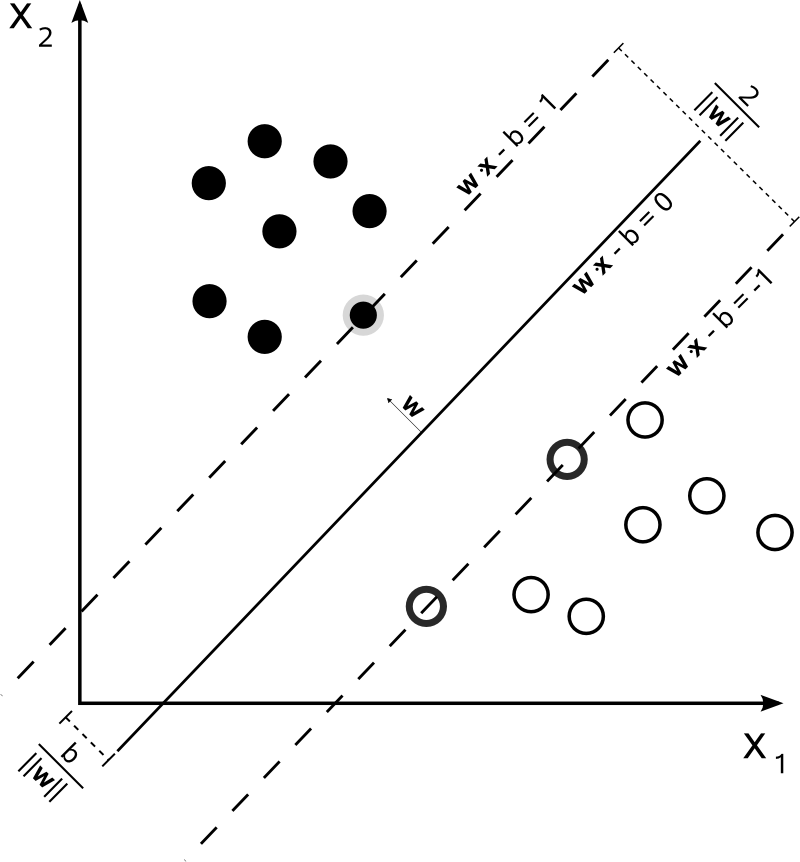
\includegraphics[width=25mm]{images/svm}
\caption{Méthode SVM pour la classification}
\label{overflow}
\end{figure}

\begin{itemize}
\item Une méthode de classification du domaine d'apprentissage automatique
\item Comment l'appliquer pour la classification d'images
\end{itemize}
\end{frame}

%=====================================================Slide 5
\begin{frame}{Processus de SVM pour la classification d'images}
\begin{enumerate}
\item Extraction des caractéristiques des images
\item Construction d'un dictionnaire a partir des caractères
\item Construction des histogrammes
\item Application SVM pour des histogrammes pour la classification
\end{enumerate}
\end{frame}

\section{État de l'art}
\subsection{Extraction des caractéristiques}
\begin{frame}{Introduction}

\end{frame}

\subsubsection{SIFT}
\begin{frame}{Méthode SIFT}

\end{frame}

\subsubsection{Sac de mots visuels}
\begin{frame}{Methode Sac de mots visuels}

\end{frame}

\subsection{Apprentissage automatique}
\begin{frame}{Introduction}

\end{frame}

\subsubsection{SVM}
\begin{frame}{Méthode SVM}

\end{frame}

\subsubsection{SGD}
\begin{frame}{Méthode SGD}

\end{frame}

\subsubsection{MCSGD}
\begin{frame}{Méthode MC-SGD}

\end{frame}

\section{Conclusion}
\begin{frame}{Conclusion}
Conclusion ici
\end{frame}

\end{otherlanguage}

% All of the following is optional and typically not needed. 
\section*{Références}

\begin{frame}
\begin{thebibliography}{9}
\bibitem{c1}
  David Lowe
  \emph{THE MNIST DATABASE of handwritten digits}.
  Yann LeCun, Courant Institute, NYU,
  Corinna Cortes, Google Labs, New York,
  Christopher J.C. Burges, Microsoft Research, Redmond,
  \emph{http://www.cs.ubc.ca/~lowe/keypoints/}
   
 
\end{thebibliography}
\end{frame}
\begin{frame}
 \Huge Merci pour votre attention!
\end{frame}

\end{document}
